% coding:utf-8

%----------------------------------------
%FOSADSVB, a LaTeX-Code for a summary of digital signal processing
%Copyright (C) 2015, Mario Felder & Michi Fallegger

%This program is free software; you can redistribute it and/or
%modify it under the terms of the GNU General Public License
%as published by the Free Software Foundation; either version 2
%of the License, or (at your option) any later version.

%This program is distributed in the hope that it will be useful,
%but WITHOUT ANY WARRANTY; without even the implied warranty of
%MERCHANTABILITY or FITNESS FOR A PARTICULAR PURPOSE.  See the
%GNU General Public License for more details.
%----------------------------------------

\chapter{Digitale Signale im Frequenzbereich}
\section{Von Fourier Tranformation zur DFT}
\subsection{Übergang zu diskreter Zeit}
Die zeitdiskrete Fourier Transformation (DTFT) kann berechnet werden mit:
\[ X(\Omega) = \sum_{n=-\infty}^{\infty} x[n]\e^{-\im\Omega n} \]
mit der normalisierten Winkelfrequenz:
\[ \Omega = 2\pi f T_S = 2\pi\frac{f}{f_S} \]
Die DTFT produziert ein $2\pi$-periodisches, kontinuierliches Spektrum.

%===============================================================================
\subsection{Übergang zu endlichem Messintervall}
Wenn nur über $N$ Abtastpunkte eine Fourier Analyse gemacht werden soll,
ist die kleinste Frequenz, welche aufgenommen werden kann:
\[ f_1 = \frac{1}{T} = \frac{1}{N \cdot T_S} = \frac{f_S}{N} \]
Die Diskrete Fourier Transformation (DFT) kann geschrieben werden als:
\[ X[k] = \sum_{n=0}^{N-1}x[n] \e^{-\im 2 \pi n \frac{k}{N}} \qquad 
	k = 0,1, 2, \ldots , N-1 \]
Die DFT ist beschränkt zu einer maximalen Frequenz von:
\[ (N-1)\frac{f_S}{N} \]
Die inverse diskrete Fourier Transformation (IDFT) ist gegeben durch:
\[ x[n] = \frac{1}{N} \sum_{k=0}^{N-1} X[k]\e^{\im 2\pi n \frac{k}{N}} 
	\qquad n = 0,1, 2, \ldots , N-1 \]
	
\begin{center}
	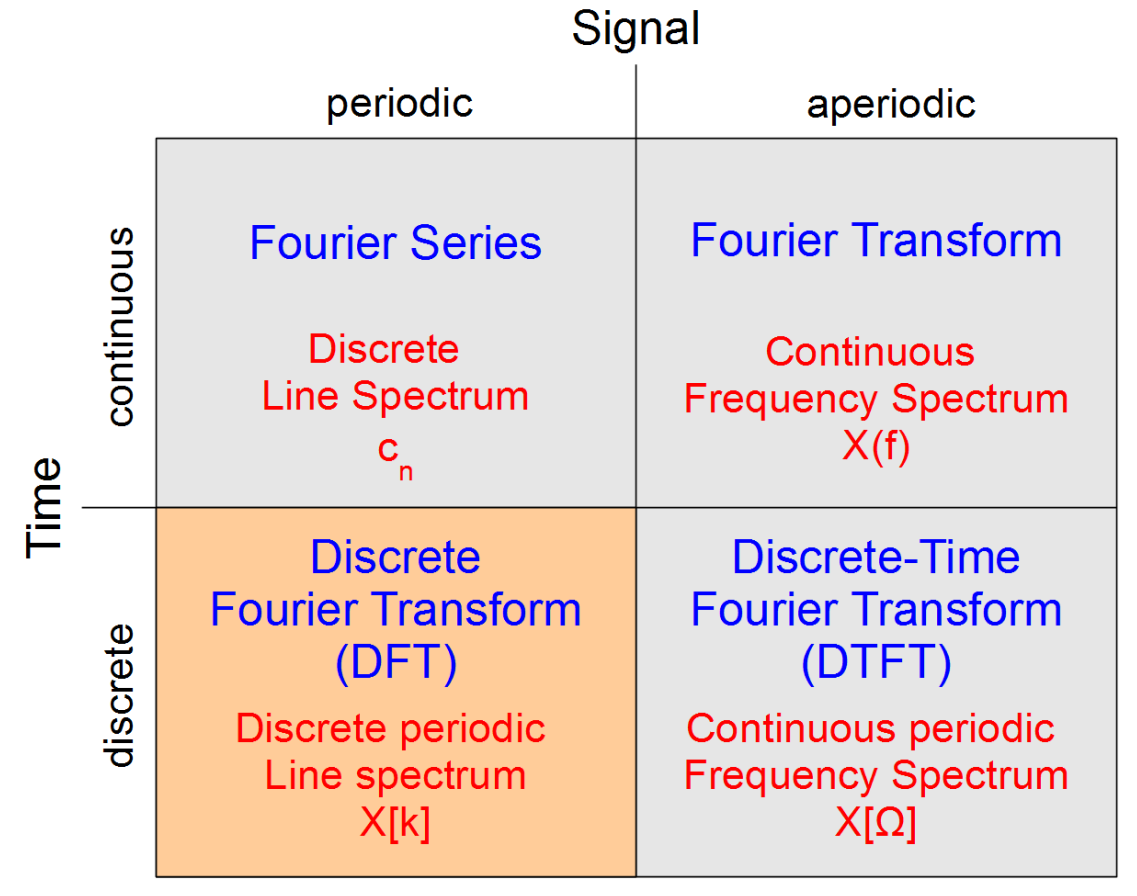
\includegraphics[scale=.7]{./images/fft_methods}
\end{center}

%===============================================================================
\section{Eingenschaften der DFT}
\textbf{Periodizität}\\
Das Spektrum der DFT ist $f_S$-periodisch
\[ X[k] = X[k+N] \]
Dementsprechend ist IDFT periodisch mit $T=NT_S$
\[ x[n] = x[n+N] \]\\
\\
\textbf{Symmetrie}\\
Die DFT eines realwertigen Signals ist symmetrisch um den Punkt $k=N/2$
\[ X[N/2+m] = X^*[N/2-m] \]\\
\\
\textbf{Zeit/Frequenz Verschiebung}\\
Verschiebung einer periodischen Zeitsequenz um $n_0$ hat einen linearen Phasen
Offset bei allen Spektralwerten zur Folge
\[ x[n+n_0] \qquad \laplace \qquad \e^{\im 2\pi n_0 \frac{k}{N}} \cdot X[k] \]
Die Multiplikation mit einem komplexen Exponent hat eine konstante
Frequenzverschiebung zur Folge
\[ \e^{\im 2\pi k_0 \frac{n}{N}} \cdot x[n] \qquad \laplace \qquad X[k-k_0] \]\\
\\
\textbf{Modulation}\\
Konsequenz der Frequenzverschiebung ist die Modulation
\[ \cos\left(2\pi k_0\frac{n}{N}\right) \cdot x[n] \qquad\laplace\qquad
	\frac{1}{2}\left( X[k+k_0] + X[k-k_0] \right) \]\\
\\
\textbf{Parseval Theorem}\\
Zwischen Signalwerten $x[k]$ und Fourier Koeffizienten $X[k]$ besteht folgende
Beziehung:
\[ \frac{1}{N} \sum_{n=0}^{N-1}x[n]^2 = \sum_{k=0}^{N-1}\left| 
	\frac{X[k]}{N} \right|^2  \]\\
\\
\textbf{Zusammenhang von Faltung und Multiplikation}\\
Punktweise Multiplikation zweier DFT Spektren $X[k]$ und $Y[k]$ im 
Frequenzbereich entspricht der zyklischen Faltung von $x[n]$ und $y[n]$ im 
Zeitbereich
\[ x[n] \circledast_N y[n] \qquad\laplace\qquad X[k]\cdot Y[k] \]

%===============================================================================
\subsection{Gültigkeitsbereich der DFT}
\[ X[k] = X[\Omega]|_{\Omega=2\pi\frac{k}{N}} \]
\textbf{$x[n]$ periodisch:}\\
Der Messintervall $NT_S$ ist ein ganzzahliger Vielfache der Periodendauer
von $x[n] $.\\
\\
\textbf{$x[n]$ aperiodisch:}\\
Alle Werte von $x[n]$ ausserhalb dem Bereich $0\geq n<N$ sind Null.

%===============================================================================
\section{Anwendungs Aspekte}
\subsection{Zero-Padding}
Um eine bessere Interpolation zwischen den $N$ Frequenzpunkten in der DFT zu
bekommen, kann das Signal im Zeitbereich mit Nullen aufgefüllt werden.
Das Spektrum $X(\Omega)$ wird nicht verändert, allerdings stehen zusätzliche
Abtastpunkte auf der Achse der normalisierten Winkelfrequenz zu Verfügung.

%===============================================================================
\subsection{Fensterfunktion}
Die DFT wendet per Definition ein Rechteckfenster an, um die $N$ Samples
auszuschneiden. Es können andere Fensterfunktionen auf das Signal $x[n]$
angewendet werden, allerdings gelten folgende Punkte:
\begin{itemize}
	\item Je schmaler die Hauptkeule im Spektrum des Fensters, desto höher ist
	die spektrale Auflösung für $X[k]$
	\item Je stärker die Dämpfung der Nebenkeulen im Spektrum des Fenster, desto
	besser die Unterdrückung der Leackage in $X[k]$
\end{itemize}

\begin{center}
	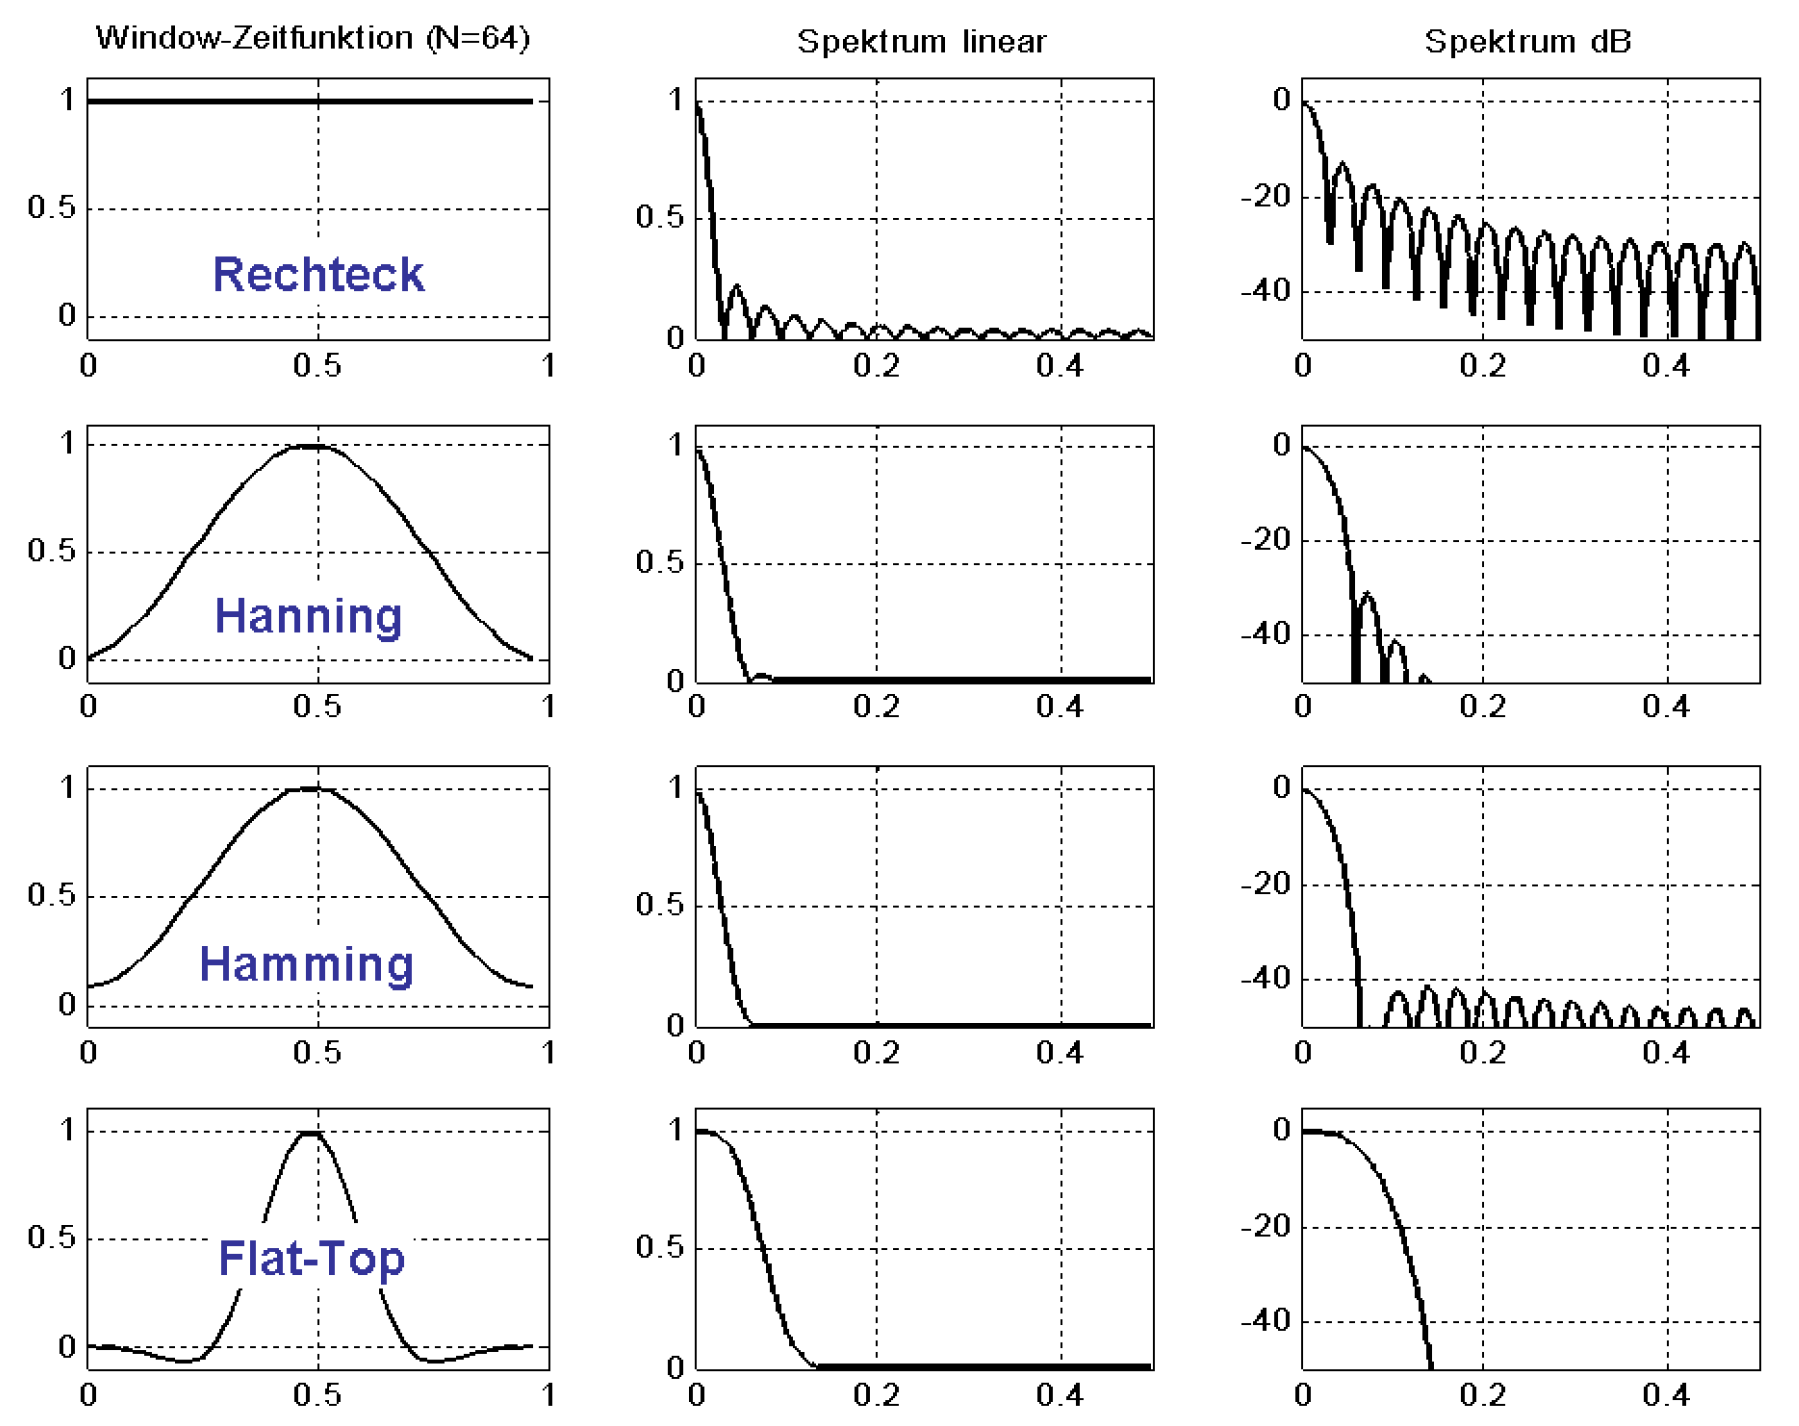
\includegraphics[scale=.7]{./images/windows}
\end{center}

%===============================================================================
\section{Short-Time DFT}
Wenn die Entwicklung des Frequenzspektrums über die Zeit interessiert, werden
kontinuierliche Berechnungen des Spektrums von kurzen Signalsektoren 
durchgeführt. Da diese kurzen Sektoren meistens nicht ein ganzzahliges
vielfache Vielfache der Periode ist, werden Fensterfunktionen angewendet.\\
\\
Bei der Länge $N$ des Fensters ergibt sich der Kompromiss von:
\begin{itemize}
	\item grosse spektrale Auflösung ($N$ gross)
	\item grosse zeitliche Auflösung ($N$ klein)
\end{itemize}

Um beides zu erreichen, können die DFT-Fenster überlappt werden um maximal
$N-1$.

%===============================================================================
\section{Fast Fourier Transformation (FFT)}
Geschwindigkeitsvergleich FFT-DFT:
\[ speedup\_factor_{FFT} = \frac{8N-2}{5\cdot \log_2N} \approx 1.5 	
	\frac{N}{\log_2N} \]
Dabei ist $N = 2^L$ mit einem ganzzahligen Wert für $L$.

%===============================================================================
\subsection{Twiddle Faktoren}
Definition:
\[ W_N = \e^{-\im\frac{2\pi}{N}} \]\\
\\
\textbf{Periodizität}\\
$W_N$ kann nur für $N$ verschiedene Zahlen ausgewertet werden. Der Twiddle
Faktor ist somit $N$-periodisch
\[ W_N^{k+N} = W_N^k \]\\
\\
\textbf{Symmetrie}\\
Abgesehen vom Vorzeichen nimmt $W_N$ nur $N/2$ verschiedene Werte an.
\[ W_N^{k+N/2} = -W_N^k \]

%===============================================================================
\subsection{Radix-2 FFT}
Die DFT wird mit dem Twiddle Faktor umgeschrieben:
\[\begin{aligned} X[k] &= \sum_{n=0}^{N-1} x[nW_N^{nk}]\\
	&= \sum_{n \textrm{ even}} x[n]W_N^{nk} + \sum_{n\textrm{ odd}}x[n]W_N^{nk}
\end{aligned}\]
Es können zwei neue Sequenzen $x_1[n]$ und $x_2[n]$ mit geraden und ungeraden
$n$ von der Länge $N/2$ erzeugt werden.
\[ X[k] = \underbrace{\sum_{n=0}^{N/2-1}x_1[n]W_{N/2}^{nk}}_{x_1[\tilde{k}]} +
	W_N^k\cdot \underbrace{\sum_{n=0}^{N/2-1} x_2[n]W_{N/2}^{nk}}_
	{{x_2[\tilde{k}]}} \]
wobei
\[ \tilde{k} = k\mod N/2 \]

\begin{center}
	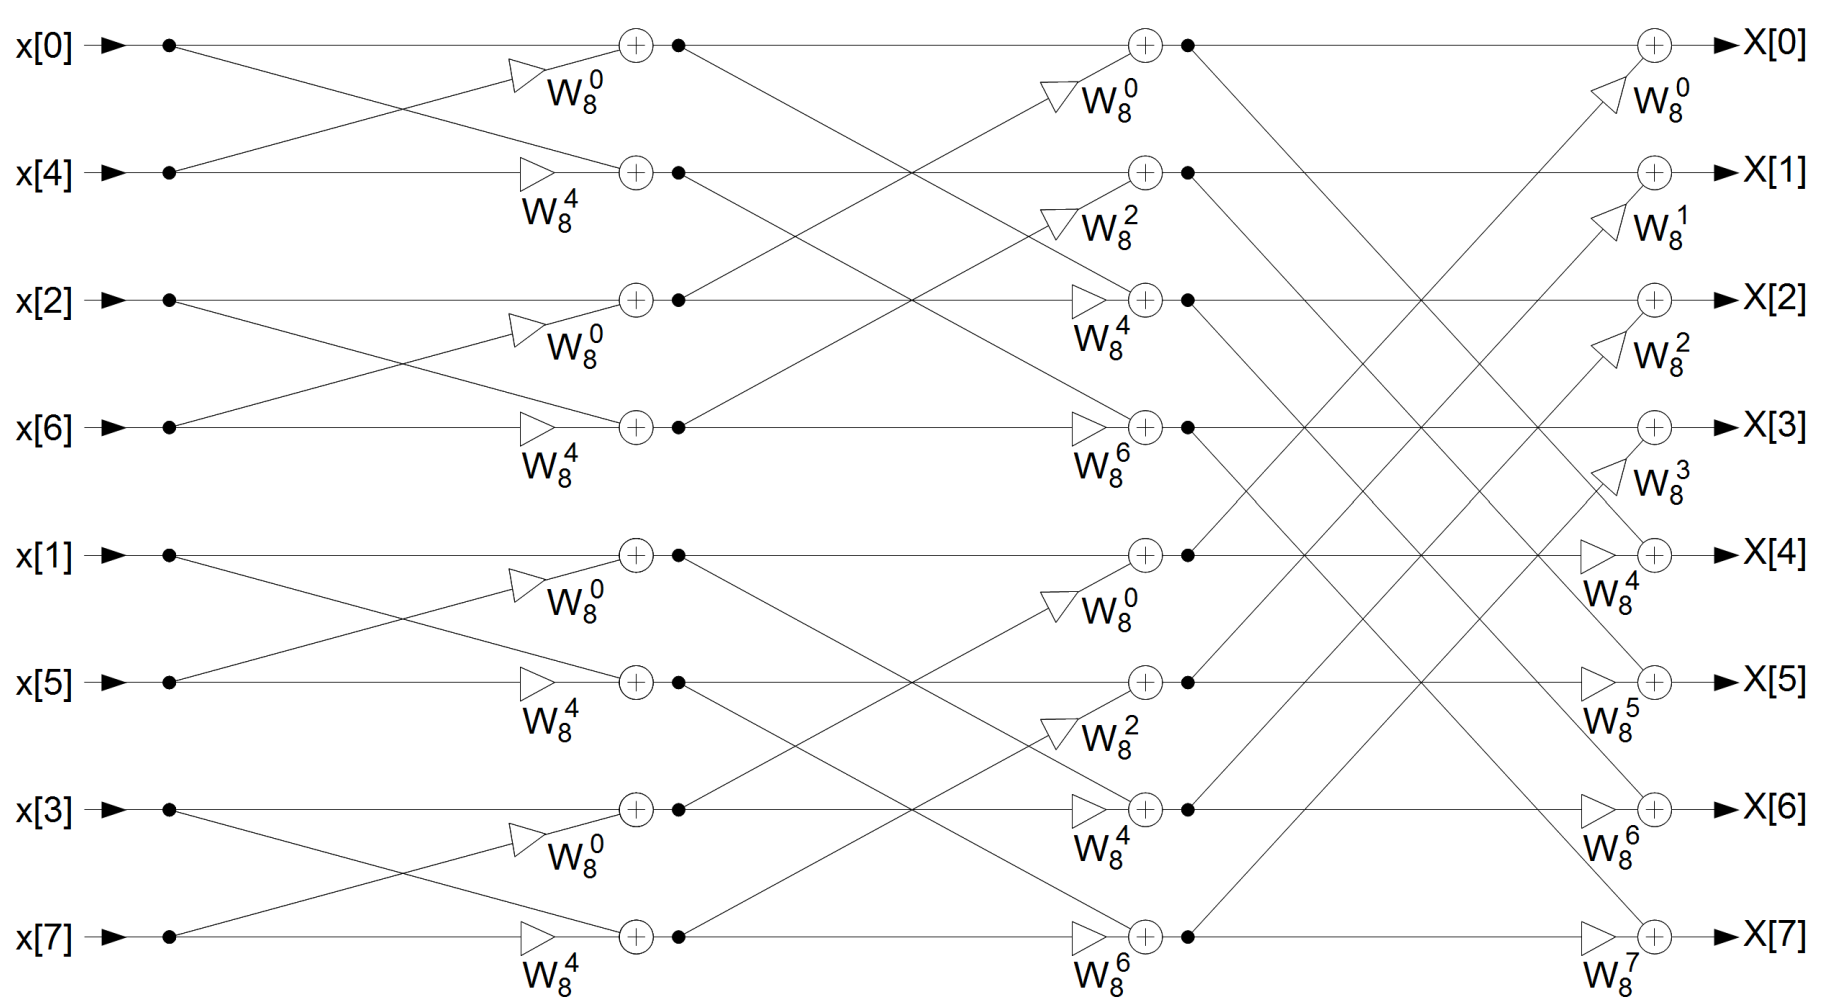
\includegraphics[scale=.7]{./images/fft}
\end{center}

Index bit-reversed in Matlab: \verb|bitrevorder|

%===============================================================================
\section{Goertzel-Algorithmus}
Definition:
\[ X[k] = y_k[n]|_{n=N} = \sum_{i=0}^{N-1}x[i]W_N^{-k(N-i)} \]
Differenzengleichung:
\[ s[n] = x[n] + a \cdot s[n-1] - s[n-2] \]
\[ y_k[n] = s[n] - W_N^k \cdot s[n-1] \]
mit 
\[ a= 2\cos 2\pi\frac{k}{N} \]
$s[n]$ muss für alle Zeitpunkte $n=0,1,\ldots,N$ berechnet werden, $y_k[n]$
nur für $n=N$.

\begin{center}
	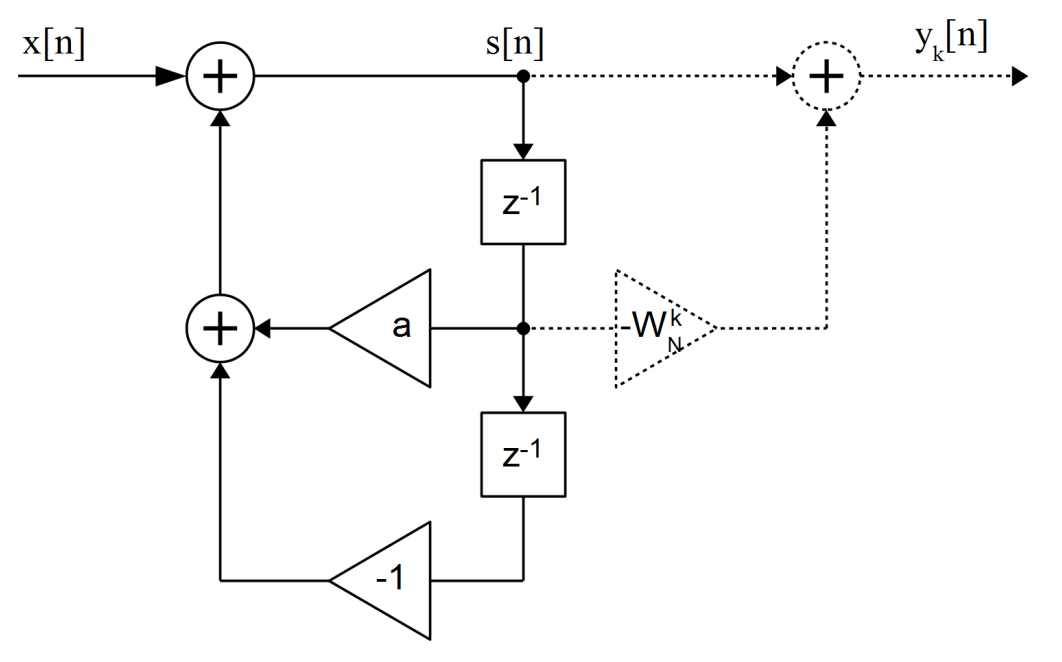
\includegraphics[scale=.7]{./images/goertzel}
\end{center}
Der Goertzel-Algorithmus gibt die DFT spectral componente bei der Frequenz
\[ f_k = k\frac{f_S}{N} \]
Mit dem PArseval Theorem kann der Leistungsgehalt $P_k$ eines realwertigen
Signals $x[n]$ bei einer Frequenz von $f_k$ ermittelt werden:
\[
	P_k = 2\left| \frac{X[k]}{N} \right|^2
		= \frac{2}{N^2}(\Re\{X[k]\}^2+\Im\{X[k]\}^2)
\]